\chapter{Training einer KI}
\label{chap:training}

In diesem Kapitel werden wir lernen, wieso und wie eine KI funktioniert.

\begin{figure}[h]
    \centering
    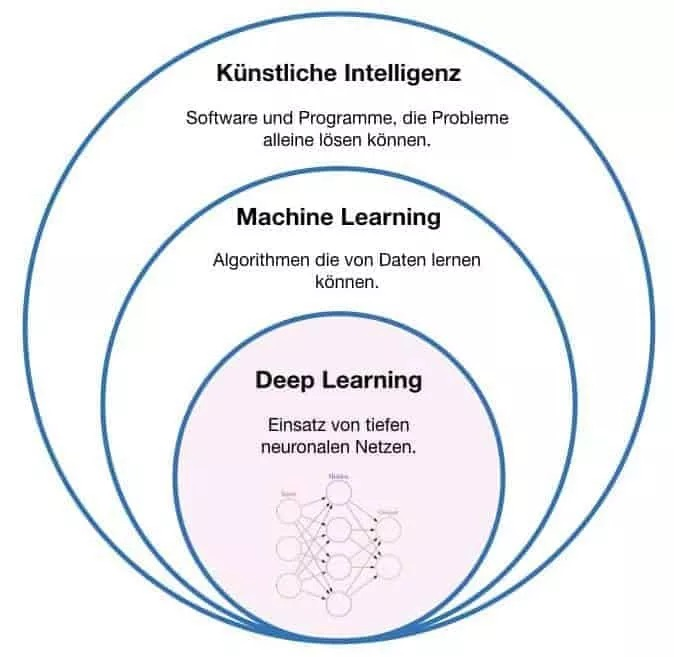
\includegraphics[width=0.5\textwidth]{ki-aufbau.jpg}
    \caption{Aufbau der KI}
    \label{fig:ki-aufbau}
\end{figure}

\section{Maschinelles Lernen}
Die KI verwendet \textbf{Maschinelles Lernen}. Damit kann der Computer automatisiert lernen. Er kann sich dabei ständig verbessern und seine Fähigkeiten verfeinern.
Für diese Methode werden Algorithmen verwendet, die Beziehungen zwischen Variablen (d. h. Muster) entdecken und dann aus diesen Lektionen lernen. Je mehr Daten sie erhalten, desto effizienter wird die KI.

\subsection{Deep Learning}
Beim \textbf{Deep Learning}-Verfahren werden \textbf{neuronale Netze} verwendet.
Neuronale Netze ahmen die Funktionsweise des menschliche Gehirns durch Algorithmen nach. Sie können aus Datenquellen Informationen und Muster erkennen und diese auf unbekannte Daten anwenden.
Das \textit{Deep Learning} wird dazu verwendet, um Bilder zu erkennen, Texte zu verstehen und Entscheidungen genauer zu tätigen.

\section{Training in drei Schritten}
Das Training einer KI ist in folgende drei Schritte aufgeteilt
.
\begin{description}
    \item[1. Training] Im ersten Schritt wird der Computer mit Daten gefüttert.
    \item[2. Validierung] kjfbosdbvlise
    \item[3. Test] ljhbfoawevfo
\end{description}

\bigskip

\section{Quellen} \citep{KI-Training}, \citep{neuronale-netze}